\section{Project Pipeline}
The project pipeline is shown in Figure \ref{fig:pipeline}, illustrating the various steps and stages involved in the automatic text summarization process. The pipeline is designed to be modular and easily extensible, allowing for the integration of new models and evaluation metrics as needed.

\begin{figure}[H]
    \centering
    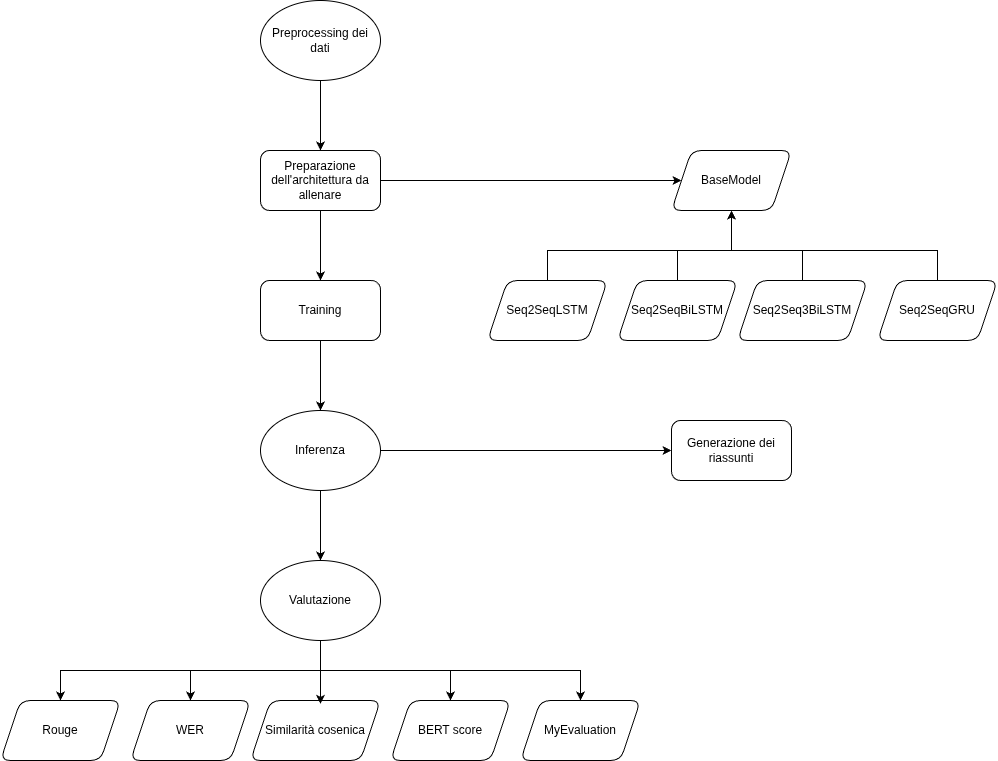
\includegraphics[width=1\textwidth]{media/pipeline.png}
    \caption{Pipeline del progetto}
    \label{fig:pipeline}
\end{figure}

The pipeline is divided into three main phases:
\begin{enumerate}
    \item \textbf{Preprocessing}: in this phase, data cleaning and preparation operations are performed, such as removing stopwords, tokenization, and text normalization.
    \item \textbf{Training}: in this phase, the summarization model is trained using the preprocessed data. A split is made between the training set and the validation set, and the model is trained using the training set while monitoring its performance on the validation set.
    \item \textbf{Evaluation}: in this phase, the summaries generated by the model are evaluated using various metrics, such as ROUGE, BERT score, and the custom metric \texttt{myevaluation}.
\end{enumerate}
In the following sections, the details of each phase of the pipeline will be explored.